\documentclass[twoside]{book}

% Packages required by doxygen
\usepackage{fixltx2e}
\usepackage{calc}
\usepackage{doxygen}
\usepackage[export]{adjustbox} % also loads graphicx
\usepackage{graphicx}
\usepackage[utf8]{inputenc}
\usepackage{makeidx}
\usepackage{multicol}
\usepackage{multirow}
\PassOptionsToPackage{warn}{textcomp}
\usepackage{textcomp}
\usepackage[nointegrals]{wasysym}
\usepackage[table]{xcolor}

% Font selection
\usepackage[T1]{fontenc}
\usepackage[scaled=.90]{helvet}
\usepackage{courier}
\usepackage{amssymb}
\usepackage{sectsty}
\renewcommand{\familydefault}{\sfdefault}
\allsectionsfont{%
  \fontseries{bc}\selectfont%
  \color{darkgray}%
}
\renewcommand{\DoxyLabelFont}{%
  \fontseries{bc}\selectfont%
  \color{darkgray}%
}
\newcommand{\+}{\discretionary{\mbox{\scriptsize$\hookleftarrow$}}{}{}}

% Page & text layout
\usepackage{geometry}
\geometry{%
  a4paper,%
  top=2.5cm,%
  bottom=2.5cm,%
  left=2.5cm,%
  right=2.5cm%
}
\tolerance=750
\hfuzz=15pt
\hbadness=750
\setlength{\emergencystretch}{15pt}
\setlength{\parindent}{0cm}
\setlength{\parskip}{3ex plus 2ex minus 2ex}
\makeatletter
\renewcommand{\paragraph}{%
  \@startsection{paragraph}{4}{0ex}{-1.0ex}{1.0ex}{%
    \normalfont\normalsize\bfseries\SS@parafont%
  }%
}
\renewcommand{\subparagraph}{%
  \@startsection{subparagraph}{5}{0ex}{-1.0ex}{1.0ex}{%
    \normalfont\normalsize\bfseries\SS@subparafont%
  }%
}
\makeatother

% Headers & footers
\usepackage{fancyhdr}
\pagestyle{fancyplain}
\fancyhead[LE]{\fancyplain{}{\bfseries\thepage}}
\fancyhead[CE]{\fancyplain{}{}}
\fancyhead[RE]{\fancyplain{}{\bfseries\leftmark}}
\fancyhead[LO]{\fancyplain{}{\bfseries\rightmark}}
\fancyhead[CO]{\fancyplain{}{}}
\fancyhead[RO]{\fancyplain{}{\bfseries\thepage}}
\fancyfoot[LE]{\fancyplain{}{}}
\fancyfoot[CE]{\fancyplain{}{}}
\fancyfoot[RE]{\fancyplain{}{\bfseries\scriptsize Generated by Doxygen }}
\fancyfoot[LO]{\fancyplain{}{\bfseries\scriptsize Generated by Doxygen }}
\fancyfoot[CO]{\fancyplain{}{}}
\fancyfoot[RO]{\fancyplain{}{}}
\renewcommand{\footrulewidth}{0.4pt}
\renewcommand{\chaptermark}[1]{%
  \markboth{#1}{}%
}
\renewcommand{\sectionmark}[1]{%
  \markright{\thesection\ #1}%
}

% Indices & bibliography
\usepackage{natbib}
\usepackage[titles]{tocloft}
\setcounter{tocdepth}{3}
\setcounter{secnumdepth}{5}
\makeindex

% Hyperlinks (required, but should be loaded last)
\usepackage{ifpdf}
\ifpdf
  \usepackage[pdftex,pagebackref=true]{hyperref}
\else
  \usepackage[ps2pdf,pagebackref=true]{hyperref}
\fi
\hypersetup{%
  colorlinks=true,%
  linkcolor=blue,%
  citecolor=blue,%
  unicode%
}

% Custom commands
\newcommand{\clearemptydoublepage}{%
  \newpage{\pagestyle{empty}\cleardoublepage}%
}

\usepackage{caption}
\captionsetup{labelsep=space,justification=centering,font={bf},singlelinecheck=off,skip=4pt,position=top}

%===== C O N T E N T S =====

\begin{document}

% Titlepage & ToC
\hypersetup{pageanchor=false,
             bookmarksnumbered=true,
             pdfencoding=unicode
            }
\pagenumbering{alph}
\begin{titlepage}
\vspace*{7cm}
\begin{center}%
{\Large Arkav\+Quarium }\\
\vspace*{1cm}
{\large Generated by Doxygen 1.8.14}\\
\end{center}
\end{titlepage}
\clearemptydoublepage
\pagenumbering{roman}
\tableofcontents
\clearemptydoublepage
\pagenumbering{arabic}
\hypersetup{pageanchor=true}

%--- Begin generated contents ---
\chapter{Arkav\+Quarium}
\label{md__r_e_a_d_m_e}
\Hypertarget{md__r_e_a_d_m_e}
tugas O\+OP 2018 
\chapter{Hierarchical Index}
\section{Class Hierarchy}
This inheritance list is sorted roughly, but not completely, alphabetically\+:\begin{DoxyCompactList}
\item \contentsline{section}{Aquarium}{\pageref{class_aquarium}}{}
\item \contentsline{section}{Entity}{\pageref{class_entity}}{}
\begin{DoxyCompactList}
\item \contentsline{section}{Guppy}{\pageref{class_guppy}}{}
\begin{DoxyCompactList}
\item \contentsline{section}{Piranha}{\pageref{class_piranha}}{}
\end{DoxyCompactList}
\item \contentsline{section}{Koin}{\pageref{class_koin}}{}
\item \contentsline{section}{Makanan}{\pageref{class_makanan}}{}
\item \contentsline{section}{Siput}{\pageref{class_siput}}{}
\end{DoxyCompactList}
\end{DoxyCompactList}

\chapter{Class Index}
\section{Class List}
Here are the classes, structs, unions and interfaces with brief descriptions\+:\begin{DoxyCompactList}
\item\contentsline{section}{\mbox{\hyperlink{class_aquarium}{Aquarium}} }{\pageref{class_aquarium}}{}
\item\contentsline{section}{\mbox{\hyperlink{class_entity}{Entity}} }{\pageref{class_entity}}{}
\item\contentsline{section}{\mbox{\hyperlink{class_guppy}{Guppy}} }{\pageref{class_guppy}}{}
\item\contentsline{section}{\mbox{\hyperlink{class_koin}{Koin}} }{\pageref{class_koin}}{}
\item\contentsline{section}{\mbox{\hyperlink{class_makanan}{Makanan}} }{\pageref{class_makanan}}{}
\item\contentsline{section}{\mbox{\hyperlink{class_piranha}{Piranha}} }{\pageref{class_piranha}}{}
\item\contentsline{section}{\mbox{\hyperlink{class_siput}{Siput}} }{\pageref{class_siput}}{}
\end{DoxyCompactList}

\chapter{Class Documentation}
\hypertarget{class_aquarium}{}\section{Aquarium Class Reference}
\label{class_aquarium}\index{Aquarium@{Aquarium}}
\subsection*{Public Member Functions}
\begin{DoxyCompactItemize}
\item 
\mbox{\Hypertarget{class_aquarium_acbf7e576e86b0bb641ff93d479936a04}\label{class_aquarium_acbf7e576e86b0bb641ff93d479936a04}} 
char {\bfseries get\+Entity} ()
\item 
\mbox{\Hypertarget{class_aquarium_ae48965035f8aa2ad3cbb54f6cbf9f34e}\label{class_aquarium_ae48965035f8aa2ad3cbb54f6cbf9f34e}} 
void {\bfseries set\+Entity} (\mbox{\hyperlink{class_entity}{Entity}})
\end{DoxyCompactItemize}


The documentation for this class was generated from the following file\+:\begin{DoxyCompactItemize}
\item 
Aquarium.\+hpp\end{DoxyCompactItemize}

\hypertarget{class_entity}{}\section{Entity Class Reference}
\label{class_entity}\index{Entity@{Entity}}


Inheritance diagram for Entity\+:
\nopagebreak
\begin{figure}[H]
\begin{center}
\leavevmode
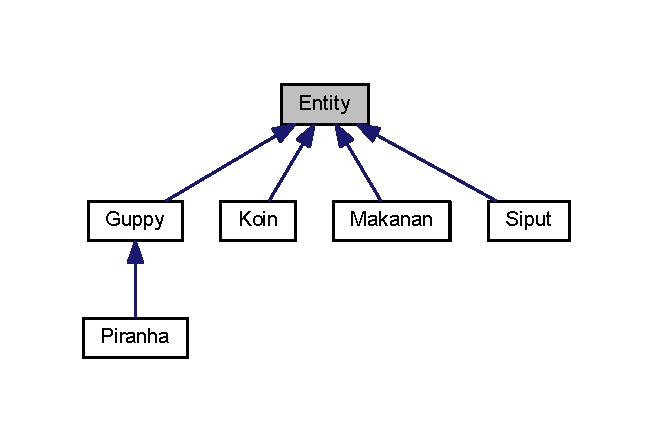
\includegraphics[width=314pt]{class_entity__inherit__graph}
\end{center}
\end{figure}
\subsection*{Public Member Functions}
\begin{DoxyCompactItemize}
\item 
\mbox{\Hypertarget{class_entity_aa7b05b89c1d319f19e06a986f6fcba8e}\label{class_entity_aa7b05b89c1d319f19e06a986f6fcba8e}} 
{\bfseries Entity} (int, int, char)
\item 
\mbox{\Hypertarget{class_entity_a8bad399d8b9c6bf23ecbb8f0b4fe6a64}\label{class_entity_a8bad399d8b9c6bf23ecbb8f0b4fe6a64}} 
int {\bfseries getX} ()
\item 
\mbox{\Hypertarget{class_entity_a4f2a264033195f9004a494069c5865f0}\label{class_entity_a4f2a264033195f9004a494069c5865f0}} 
int {\bfseries getY} ()
\item 
\mbox{\Hypertarget{class_entity_adef8f8f46bf832bf07fe5b91cc808e3b}\label{class_entity_adef8f8f46bf832bf07fe5b91cc808e3b}} 
char {\bfseries get\+Kind} ()
\item 
\mbox{\Hypertarget{class_entity_a3fbf5396e39940e060e48e1c298992dc}\label{class_entity_a3fbf5396e39940e060e48e1c298992dc}} 
void {\bfseries setX} (int)
\item 
\mbox{\Hypertarget{class_entity_a2241bb3600829d1c3f28577fecf739af}\label{class_entity_a2241bb3600829d1c3f28577fecf739af}} 
void {\bfseries setY} (int)
\item 
\mbox{\Hypertarget{class_entity_aa9cdd93807cbc1b39e7afc95110deb60}\label{class_entity_aa9cdd93807cbc1b39e7afc95110deb60}} 
void {\bfseries set\+Kind} (char)
\item 
\mbox{\Hypertarget{class_entity_a624e85b5e363a70b0a7b2e04912c6cdf}\label{class_entity_a624e85b5e363a70b0a7b2e04912c6cdf}} 
virtual void {\bfseries move} ()=0
\end{DoxyCompactItemize}
\subsection*{Protected Attributes}
\begin{DoxyCompactItemize}
\item 
\mbox{\Hypertarget{class_entity_aed19b548bf7e959c6e6443bd86e95663}\label{class_entity_aed19b548bf7e959c6e6443bd86e95663}} 
int {\bfseries posX}
\item 
\mbox{\Hypertarget{class_entity_a68f5b79639fd7aca3a17cacf16dcf028}\label{class_entity_a68f5b79639fd7aca3a17cacf16dcf028}} 
int {\bfseries posY}
\end{DoxyCompactItemize}


The documentation for this class was generated from the following file\+:\begin{DoxyCompactItemize}
\item 
Entity.\+hpp\end{DoxyCompactItemize}

\hypertarget{class_guppy}{}\section{Guppy Class Reference}
\label{class_guppy}\index{Guppy@{Guppy}}


Inheritance diagram for Guppy\+:
\nopagebreak
\begin{figure}[H]
\begin{center}
\leavevmode
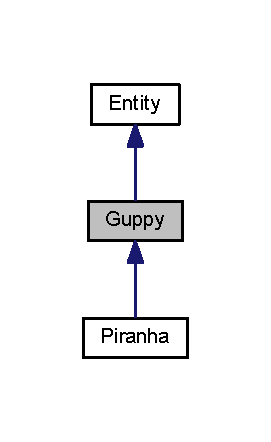
\includegraphics[width=130pt]{class_guppy__inherit__graph}
\end{center}
\end{figure}


Collaboration diagram for Guppy\+:
\nopagebreak
\begin{figure}[H]
\begin{center}
\leavevmode
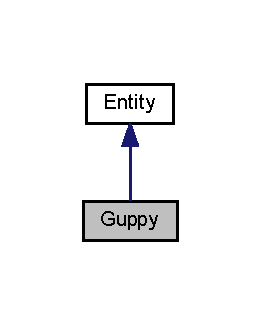
\includegraphics[width=125pt]{class_guppy__coll__graph}
\end{center}
\end{figure}
\subsection*{Public Member Functions}
\begin{DoxyCompactItemize}
\item 
\mbox{\Hypertarget{class_guppy_a28662f8f82c743d7c01deac586e6ca5e}\label{class_guppy_a28662f8f82c743d7c01deac586e6ca5e}} 
{\bfseries Guppy} (int, int, int, int)
\item 
\mbox{\Hypertarget{class_guppy_a60e492213ba14f89484b9f26c0a6a414}\label{class_guppy_a60e492213ba14f89484b9f26c0a6a414}} 
int {\bfseries get\+Level} ()
\item 
\mbox{\Hypertarget{class_guppy_a7567664b093759516cd155a1764847e6}\label{class_guppy_a7567664b093759516cd155a1764847e6}} 
bool {\bfseries is\+Kenyang} ()
\item 
\mbox{\Hypertarget{class_guppy_a49961b1bcd93d43496f081d1732ddce8}\label{class_guppy_a49961b1bcd93d43496f081d1732ddce8}} 
bool {\bfseries is\+Lapar} ()
\item 
\mbox{\Hypertarget{class_guppy_aa9a5c199be094098529c973ba403087e}\label{class_guppy_aa9a5c199be094098529c973ba403087e}} 
void {\bfseries set\+Level} (int)
\item 
\mbox{\Hypertarget{class_guppy_ac8ff64e3a7e8ea83284971ef698d8823}\label{class_guppy_ac8ff64e3a7e8ea83284971ef698d8823}} 
void {\bfseries set\+Kenyang} (int)
\item 
\mbox{\Hypertarget{class_guppy_adcf0c39769a6bfd1c3046af0d464b3a8}\label{class_guppy_adcf0c39769a6bfd1c3046af0d464b3a8}} 
virtual void {\bfseries find\+Food} ()
\item 
\mbox{\Hypertarget{class_guppy_ae6002948d74b3741bed34a7311be4377}\label{class_guppy_ae6002948d74b3741bed34a7311be4377}} 
void {\bfseries move} ()
\item 
\mbox{\Hypertarget{class_guppy_ad67e3b60be4e541b15e90b9e6581a920}\label{class_guppy_ad67e3b60be4e541b15e90b9e6581a920}} 
virtual {\bfseries drop\+Coin} ()
\end{DoxyCompactItemize}
\subsection*{Protected Attributes}
\begin{DoxyCompactItemize}
\item 
\mbox{\Hypertarget{class_guppy_aad3ed21afd22dd1ff36bcbe3e3e9022f}\label{class_guppy_aad3ed21afd22dd1ff36bcbe3e3e9022f}} 
int {\bfseries level}
\item 
\mbox{\Hypertarget{class_guppy_aa02c8accc01fc84c6f9d38d128912f4e}\label{class_guppy_aa02c8accc01fc84c6f9d38d128912f4e}} 
int {\bfseries kenyang}
\end{DoxyCompactItemize}


The documentation for this class was generated from the following file\+:\begin{DoxyCompactItemize}
\item 
Guppy.\+hpp\end{DoxyCompactItemize}

\hypertarget{class_koin}{}\section{Koin Class Reference}
\label{class_koin}\index{Koin@{Koin}}


Inheritance diagram for Koin\+:
\nopagebreak
\begin{figure}[H]
\begin{center}
\leavevmode
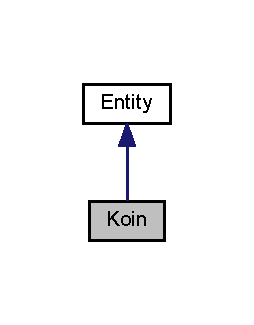
\includegraphics[width=122pt]{class_koin__inherit__graph}
\end{center}
\end{figure}


Collaboration diagram for Koin\+:
\nopagebreak
\begin{figure}[H]
\begin{center}
\leavevmode
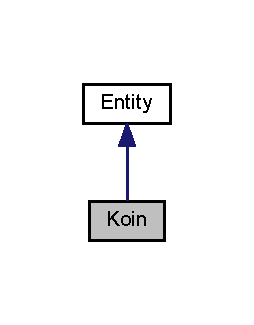
\includegraphics[width=122pt]{class_koin__coll__graph}
\end{center}
\end{figure}
\subsection*{Public Member Functions}
\begin{DoxyCompactItemize}
\item 
\mbox{\Hypertarget{class_koin_a68434ca0d1c219f1863e9d43bc9a0be4}\label{class_koin_a68434ca0d1c219f1863e9d43bc9a0be4}} 
{\bfseries Koin} (int, int, int)
\item 
\mbox{\Hypertarget{class_koin_a086d48dfd240ab4a139e0c97e8b7fb04}\label{class_koin_a086d48dfd240ab4a139e0c97e8b7fb04}} 
void {\bfseries move} ()
\end{DoxyCompactItemize}
\subsection*{Additional Inherited Members}


The documentation for this class was generated from the following file\+:\begin{DoxyCompactItemize}
\item 
Koin.\+hpp\end{DoxyCompactItemize}

\hypertarget{class_makanan}{}\section{Makanan Class Reference}
\label{class_makanan}\index{Makanan@{Makanan}}


Inheritance diagram for Makanan\+:
\nopagebreak
\begin{figure}[H]
\begin{center}
\leavevmode
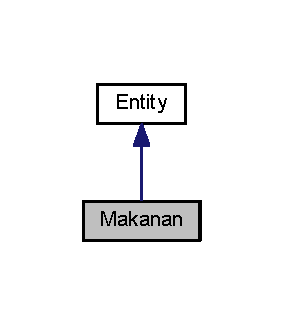
\includegraphics[width=136pt]{class_makanan__inherit__graph}
\end{center}
\end{figure}


Collaboration diagram for Makanan\+:
\nopagebreak
\begin{figure}[H]
\begin{center}
\leavevmode
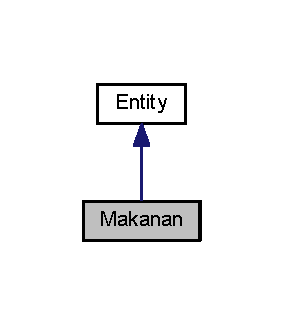
\includegraphics[width=136pt]{class_makanan__coll__graph}
\end{center}
\end{figure}
\subsection*{Public Member Functions}
\begin{DoxyCompactItemize}
\item 
\mbox{\Hypertarget{class_makanan_aa3e4801d7e413401c502e1b6fa4e994a}\label{class_makanan_aa3e4801d7e413401c502e1b6fa4e994a}} 
{\bfseries Makanan} (int, int)
\item 
\mbox{\Hypertarget{class_makanan_a02f224d8090f673bb67a2191d3b992ae}\label{class_makanan_a02f224d8090f673bb67a2191d3b992ae}} 
void {\bfseries move} ()
\end{DoxyCompactItemize}
\subsection*{Additional Inherited Members}


The documentation for this class was generated from the following file\+:\begin{DoxyCompactItemize}
\item 
Makanan.\+hpp\end{DoxyCompactItemize}

\hypertarget{class_piranha}{}\section{Piranha Class Reference}
\label{class_piranha}\index{Piranha@{Piranha}}


Inheritance diagram for Piranha\+:
\nopagebreak
\begin{figure}[H]
\begin{center}
\leavevmode
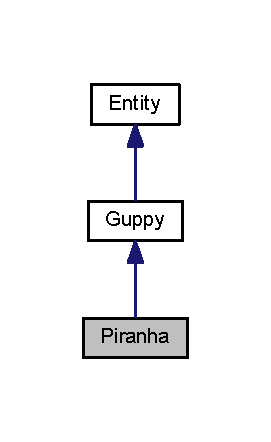
\includegraphics[width=130pt]{class_piranha__inherit__graph}
\end{center}
\end{figure}


Collaboration diagram for Piranha\+:
\nopagebreak
\begin{figure}[H]
\begin{center}
\leavevmode
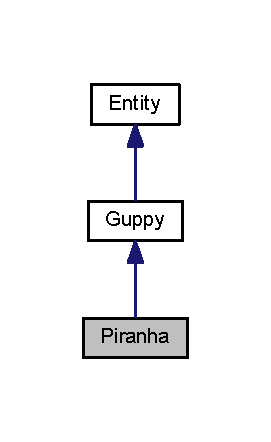
\includegraphics[width=130pt]{class_piranha__coll__graph}
\end{center}
\end{figure}
\subsection*{Public Member Functions}
\begin{DoxyCompactItemize}
\item 
\mbox{\Hypertarget{class_piranha_a51163ce0eb4f08fe46375b19055b4a13}\label{class_piranha_a51163ce0eb4f08fe46375b19055b4a13}} 
{\bfseries Piranha} (int, int, int, int)
\item 
\mbox{\Hypertarget{class_piranha_a84231f6989880f186bf64e768e68289c}\label{class_piranha_a84231f6989880f186bf64e768e68289c}} 
void {\bfseries find\+Food} ()
\item 
\mbox{\Hypertarget{class_piranha_aee107987f36631002f04c5283564382b}\label{class_piranha_aee107987f36631002f04c5283564382b}} 
void {\bfseries drop\+Coin} ()
\end{DoxyCompactItemize}
\subsection*{Additional Inherited Members}


The documentation for this class was generated from the following file\+:\begin{DoxyCompactItemize}
\item 
Piranha.\+hpp\end{DoxyCompactItemize}

\hypertarget{class_siput}{}\section{Siput Class Reference}
\label{class_siput}\index{Siput@{Siput}}


Inheritance diagram for Siput\+:
\nopagebreak
\begin{figure}[H]
\begin{center}
\leavevmode
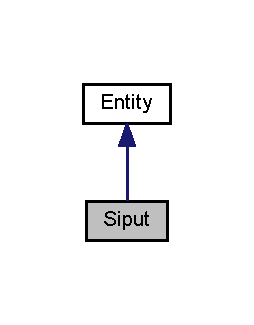
\includegraphics[width=122pt]{class_siput__inherit__graph}
\end{center}
\end{figure}


Collaboration diagram for Siput\+:
\nopagebreak
\begin{figure}[H]
\begin{center}
\leavevmode
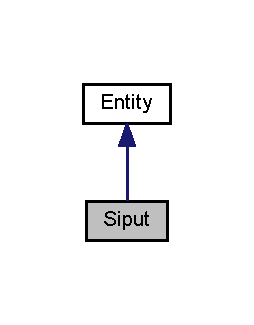
\includegraphics[width=122pt]{class_siput__coll__graph}
\end{center}
\end{figure}
\subsection*{Public Member Functions}
\begin{DoxyCompactItemize}
\item 
\mbox{\Hypertarget{class_siput_abbbf9701e21784f1e08d3c3aa92c0105}\label{class_siput_abbbf9701e21784f1e08d3c3aa92c0105}} 
{\bfseries Siput} (int, int)
\item 
\mbox{\Hypertarget{class_siput_a4f5cceefab1fdfb494c7eebaabcd0300}\label{class_siput_a4f5cceefab1fdfb494c7eebaabcd0300}} 
void {\bfseries get\+Coin} ()
\item 
\mbox{\Hypertarget{class_siput_a40de61cd661fe26389b4f53e071e44d4}\label{class_siput_a40de61cd661fe26389b4f53e071e44d4}} 
void {\bfseries move} ()
\end{DoxyCompactItemize}
\subsection*{Additional Inherited Members}


The documentation for this class was generated from the following file\+:\begin{DoxyCompactItemize}
\item 
Siput.\+hpp\end{DoxyCompactItemize}

%--- End generated contents ---

% Index
\backmatter
\newpage
\phantomsection
\clearemptydoublepage
\addcontentsline{toc}{chapter}{Index}
\printindex

\end{document}
